\documentclass{article}
\RequirePackage{amsmath}
\RequirePackage{bytefield}
\RequirePackage{graphicx}
\RequirePackage{newtxmath}
\RequirePackage{mathtools}
\RequirePackage{xspace}
\RequirePackage{url}
\RequirePackage{changepage}
\RequirePackage{lmodern}

\setlength{\oddsidemargin}{-0.25in} % Left margin of 1 in + 0 in = 1 in
\setlength{\textwidth}{7in}   % Right margin of 8.5 in - 1 in - 6.5 in = 1 in
\setlength{\topmargin}{-.75in}  % Top margin of 2 in -0.75 in = 1 in
\setlength{\textheight}{9.2in}  % Lower margin of 11 in - 9 in - 1 in = 1 in
\setlength{\parskip}{1.5ex}
\setlength{\parindent}{0ex}

\mathchardef\mhyphen="2D

\RequirePackage[usenames,dvipsnames]{xcolor}
% https://en.wikibooks.org/wiki/LaTeX/Colors#The_68_standard_colors_known_to_dvips
\newcommand{\eli}[1]{{\color{JungleGreen}\sf{Eli: #1}}}
\newcommand{\sean}[1]{{\color{blue}\sf{Sean: #1}}}
\newcommand{\taylor}[1]{{\color{red}\sf{Taylor: #1}}}
\newcommand{\daira}[1]{{\color{RedOrange}\sf{Daira: #1}}}
\newcommand{\nathan}[1]{{\color{ForestGreen}\sf{Nathan: #1}}}
\newcommand{\todo}[1]{{\color{Sepia}\sf{TODO: #1}}}

\newcommand{\changedcolor}{magenta}
\newcommand{\setchanged}{\color{\changedcolor}}
\newcommand{\changed}[1]{{\setchanged{#1}}}

% terminology

\newcommand{\term}[1]{\textsl{#1}\xspace}
\newcommand{\termbf}[1]{\textbf{#1}\xspace}

\newcommand{\Zcash}{\termbf{Zcash}}
\newcommand{\Zerocash}{\termbf{Zerocash}}
\newcommand{\Bitcoin}{\termbf{Bitcoin}}
\newcommand{\ZEC}{\termbf{ZEC}}
\newcommand{\zatoshi}{\term{zatoshi}}

\newcommand{\coin}{\term{coin}}
\newcommand{\coins}{\term{coins}}
\newcommand{\coinCommitment}{\term{coin commitment}}
\newcommand{\coinCommitments}{\term{coin commitments}}
\newcommand{\coinCommitmentTree}{\term{coin commitment tree}}
\newcommand{\PourDescription}{\term{Pour description}}
\newcommand{\PourDescriptions}{\term{Pour descriptions}}
\newcommand{\sequenceOfPourDescriptions}{\changed{sequence of} \PourDescription\changed{\term{s}}}
\newcommand{\PourTransfer}{\term{Pour transfer}}
\newcommand{\PourTransfers}{\term{Pour transfers}}
\newcommand{\fullnode}{\term{full node}}
\newcommand{\fullnodes}{\term{full nodes}}
\newcommand{\anchor}{\term{anchor}}
\newcommand{\anchors}{\term{anchors}}
\newcommand{\block}{\term{block}}
\newcommand{\blocks}{\term{blocks}}
\newcommand{\transaction}{\term{transaction}}
\newcommand{\transactions}{\term{transactions}}
\newcommand{\blockchainview}{\term{blockchain view}}
\newcommand{\mempool}{\term{mempool}}
\newcommand{\treestate}{\term{treestate}}
\newcommand{\treestates}{\term{treestates}}
\newcommand{\script}{\term{script}}
\newcommand{\serialNumber}{\term{serial number}}
\newcommand{\serialNumbers}{\term{serial numbers}}
\newcommand{\publicAddress}{\term{confidential address}}
% Let's rename ``privateAddress'' to something else, since it sounds like an oxymoron to me. (This is related to a code naming issue #602 and we might want to update both at the same time.)
\newcommand{\privateAddress}{\term{confidential private key}}
\newcommand{\coinPlaintext}{\term{coin plaintext}}
\newcommand{\coinPlaintexts}{\term{coin plaintexts}}
\newcommand{\coinsCiphertext}{\term{transmitted coins ciphertext}}
\newcommand{\transmitPublicAlgorithm}{\term{key-private encryption}}
\newcommand{\transmitPrivateAlgorithm}{\term{key-private decryption}}
\newcommand{\spendAuthority}{\term{spend authority}}
\newcommand{\incrementalMerkleTree}{\term{incremental merkle tree}}
\newcommand{\spentSerialsMap}{\term{spent serial numbers map}}
\newcommand{\zkSNARK}{\term{zk-SNARK}}
\newcommand{\zkSNARKs}{\term{zk-SNARKs}}
\newcommand{\memo}{\term{memo field}}

% key pairs:
\newcommand{\PublicAddress}{\mathsf{addr_{pk}}}
\newcommand{\PrivateAddress}{\mathsf{addr_{sk}}}
\newcommand{\PublicAddressLeadByte}{\mathbf{0x92}}
\newcommand{\PrivateAddressLeadByte}{\mathbf{0x93}}
\newcommand{\SpendAuthorityPublic}{\mathsf{a_{pk}}}
\newcommand{\SpendAuthorityPrivate}{\mathsf{a_{sk}}}
\newcommand{\SpendAuthorityPublicOld}[1]{\mathsf{a^{old}_{pk,\mathnormal{#1}}}}
\newcommand{\SpendAuthorityPrivateOld}[1]{\mathsf{a^{old}_{sk,\mathnormal{#1}}}}
\newcommand{\SpendAuthorityPublicNew}[1]{\mathsf{a^{new}_{pk,\mathnormal{#1}}}}
\newcommand{\SpendAuthorityPrivateNew}[1]{\mathsf{a^{new}_{sk,\mathnormal{#1}}}}
\newcommand{\TransmitPublic}{\mathsf{pk_{enc}}}
\newcommand{\TransmitPublicNew}[1]{\mathsf{pk_{enc,\mathnormal{#1}}}}
\newcommand{\TransmitPrivate}{\mathsf{sk_{enc}}}
\newcommand{\TransmitPrivateNew}[1]{\mathsf{sk_{enc,\mathnormal{#1}}}}
\newcommand{\EphemeralPublic}{\mathsf{pk_{eph}}}
\newcommand{\EphemeralPrivate}{\mathsf{sk_{eph}}}
\newcommand{\Value}{\mathsf{v}}

% Coins
\newcommand{\Coin}{\mathbf{c}}
\newcommand{\CoinCommitRand}{\mathsf{r}}
\newcommand{\CoinCommitRandOld}[1]{\mathsf{r^{old}_\mathnormal{#1}}}
\newcommand{\CoinCommitRandNew}[1]{\mathsf{r^{new}_\mathnormal{#1}}}
\newcommand{\CoinAddressRand}{\mathsf{\uprho}}
\newcommand{\CoinAddressRandOld}[1]{\mathsf{\uprho^{old}_\mathnormal{#1}}}
\newcommand{\CoinAddressRandNew}[1]{\mathsf{\uprho^{new}_\mathnormal{#1}}}
\newcommand{\CoinAddressPreRand}{\mathsf{\upvarphi}}
\newcommand{\CoinCommitS}{\mathsf{s}}
\newcommand{\TransmitPlaintextVersionByte}{\mathbf{0x00}}
\newcommand{\hSigInputVersionByte}{\mathbf{0x00}}
\newcommand{\Memo}{\mathsf{memo}}
\newcommand{\CryptoBox}{\mathsf{crypto\_box}}
\newcommand{\CryptoBoxOpen}{\mathsf{crypto\_box\_open}}
\newcommand{\CryptoBoxSeal}{\mathsf{crypto\_box\_seal}}
\newcommand{\CryptoBoxSpecific}{\mathsf{crypto\_box\_curve25519xsalsa20poly1305}}
\newcommand{\Plaintext}[1]{\mathbf{P}_{#1}}
\newcommand{\Ciphertext}[1]{\mathbf{C}_{#1}}
\newcommand{\Nonce}{\mathsf{nonce}}
\newcommand{\Prenonce}{\mathsf{prenonce}}
\newcommand{\TransmitEncrypt}[1]{\mathsf{Encrypt}_{#1}}
\newcommand{\TransmitDecrypt}[1]{\mathsf{Decrypt}_{#1}}
\newcommand{\CRH}{\mathsf{CRH}}
\newcommand{\CRHbox}[1]{\CRH\left(\;\raisebox{-1.3ex}{\usebox{#1}}\;\right)}
\newcommand{\FullHash}{\mathtt{SHA256}}
\newcommand{\FullHashbox}[1]{\FullHash\left(\;\raisebox{-1.3ex}{\usebox{#1}}\;\right)}
\newcommand{\Justthebox}[1]{\;\raisebox{-1.3ex}{\usebox{#1}}\;}
\newcommand{\PRF}[2]{\mathsf{{PRF}^{#2}_\mathnormal{#1}}}
\newcommand{\PRFaddr}[1]{\PRF{#1}{addr}}
\newcommand{\PRFsn}[1]{\PRF{#1}{sn}}
\newcommand{\PRFpk}[1]{\PRF{#1}{pk}}
\newcommand{\PRFrho}[1]{\PRF{#1}{\CoinAddressRand}}
\newcommand{\SHA}{\mathtt{SHA256Compress}}
\newcommand{\SHAName}{\term{SHA-256 compression}}
\newcommand{\SHAOrig}{\term{SHA-256}}
\newcommand{\cm}{\mathsf{cm}}
\newcommand{\cmNew}[1]{\mathsf{{cm}^{new}_\mathnormal{#1}}}
\newcommand{\InternalHashK}{\mathsf{k}}
\newcommand{\InternalHash}{\mathsf{InternalH}}
\newcommand{\Leading}[1]{\mathtt{Leading}_{#1}}
\newcommand{\ReplacementCharacter}{\textsf{U+FFFD}}

% merkle tree
\newcommand{\MerkleDepth}{\mathsf{d}}
\newcommand{\sn}{\mathsf{sn}}
\newcommand{\snOld}[1]{\mathsf{{sn}^{old}_\mathnormal{#1}}}

% bitcoin
\newcommand{\vin}{\mathtt{vin}}
\newcommand{\vout}{\mathtt{vout}}
\newcommand{\vpour}{\mathtt{vpour}}
\newcommand{\vpubOldField}{\mathtt{vpub\_old}}
\newcommand{\vpubNewField}{\mathtt{vpub\_new}}
\newcommand{\vsum}[2]{\smashoperator[r]{\sum_{#1}^{#2}}}
\newcommand{\anchorField}{\mathtt{anchor}}
\newcommand{\scriptSig}{\mathtt{scriptSig}}
\newcommand{\scriptPubKey}{\mathtt{scriptPubKey}}
\newcommand{\serials}{\mathtt{serials}}
\newcommand{\commitments}{\mathtt{commitments}}
\newcommand{\ephemeralKey}{\mathtt{ephemeralKey}}
\newcommand{\ciphertexts}{\mathtt{ciphertexts}}
\newcommand{\rt}{\mathsf{rt}}

% pour
\newcommand{\hSig}{\mathsf{h_{Sig}}}
\newcommand{\h}[1]{\mathsf{h_{\mathnormal{#1}}}}
\newcommand{\NOld}{\mathrm{N}^\mathsf{old}}
\newcommand{\NNew}{\mathrm{N}^\mathsf{new}}
\newcommand{\vmacs}{\mathtt{vmacs}}
\newcommand{\zkproof}{\mathtt{zkproof}}
\newcommand{\PourCircuit}{\term{\texttt{POUR} circuit}}
\newcommand{\PourStatement}{\texttt{POUR}}
\newcommand{\PourProof}{\pi_{\PourStatement}}
\newcommand{\vpubOld}{\mathsf{v_{pub}^{old}}}
\newcommand{\vpubNew}{\mathsf{v_{pub}^{new}}}
\newcommand{\cOld}[1]{\mathbf{c}_{#1}^\mathsf{old}}
\newcommand{\cNew}[1]{\mathbf{c}_{#1}^\mathsf{new}}
\newcommand{\vOld}[1]{\mathsf{v}_{#1}^\mathsf{old}}
\newcommand{\vNew}[1]{\mathsf{v}_{#1}^\mathsf{new}}
\newcommand{\NP}{\mathsf{NP}}
\newcommand{\treepath}[1]{\mathsf{path}_{#1}}
\newcommand{\COMM}[1]{\mathsf{COMM}_{#1}}
\newcommand{\COMMtrapdoor}{\term{\textsf{COMM} trapdoor}}
\newcommand{\CoinCommitment}[1]{\mathtt{CoinCommitment}(#1)}


\begin{document}

\title{Zcash Protocol Specification}
%\subtitle{Version: 2.0-draft}
\author{Sean Bowe | Daira Hopwood | Taylor Hornby}
\date{\today}
\maketitle
\section{Introduction}

\Zcash is an implementation of the \term{Decentralized Anonymous Payment}
scheme \Zerocash \cite{ZerocashOakland} with some adjustments to terminology,
functionality and performance. It bridges the existing \emph{transparent}
payment scheme used by \Bitcoin with a \emph{confidential} payment scheme
protected by zero-knowledge succinct non-interactive arguments of knowledge
(\zkSNARKs).

Changes from the original \Zerocash are highlighted in \changed{\changedcolor}.

\section{Concepts}

\subsection{Integers, Bit Sequences, and Endianness}

All integers visible in \Zcash-specific encodings are unsigned, have a fixed
bit length, and are encoded as big-endian.

In bit layout diagrams, each box of the diagram represents a sequence of bits.
If the content of the box is a byte sequence, it is implicitly converted to
a sequence of bits using big endian order. The bit sequences are then
concatenated in the order shown from left to right, and the result is converted
to a sequence of bytes, again using big-endian order.

\nathan{An example would help here. It would be illustrative if it had
a few differently-sized fields.}

$\Leading{k}(x)$, where $k$ is an integer and $x$ is a bit sequence, returns
the leading (initial) $k$ bits of its input.

\subsection{Cryptographic Functions}

$\CRH$ is a collision-resistant hash function. In \Zcash, the $\SHAName$ function
is used which takes a 512-bit block and produces a 256-bit hash. This is
different from the $\SHAOrig$ function, which hashes arbitrary-length strings.
\cite{sha256}

$\PRF{x}{}$ is a pseudo-random function seeded by $x$. Four \emph{independent}
$\PRF{x}{}$ are needed in our scheme: $\PRFaddr{x}$, $\PRFsn{x}$, $\PRFpk{x}$, and
$\PRFrho{x}$. It is required that $\PRFsn{x}$ and $\PRFrho{x}$ be
collision-resistant across all $x$ --- i.e. it should not be feasible to find
$(x, y) \neq (x', y')$ such that $\PRFsn{x}(y) = \PRFsn{x'}(y')$, and similarly
for $\PRFrho{}$.

In \Zcash, the $\SHAName$ function is used to construct all four of these
functions. The bits $\mathtt{00}$, $\mathtt{01}$, $\mathtt{10}$, and $\mathtt{11}$
are included (respectively) within the blocks that are hashed, ensuring that the
functions are independent.

\newsavebox{\addrbox}
\begin{lrbox}{\addrbox}
\begin{bytefield}[bitwidth=0.065em]{512}
        \bitbox{242}{256 bit $\SpendAuthorityPrivate$} &
        \bitbox{14}{0} &
        \bitbox{14}{0} &
        \bitbox{242}{$0^{254}$} &
\end{bytefield}
\end{lrbox}

\newsavebox{\snbox}
\begin{lrbox}{\snbox}
\begin{bytefield}[bitwidth=0.065em]{512}
        \bitbox{242}{256 bit $\SpendAuthorityPrivate$} &
        \bitbox{14}{0} &
        \bitbox{14}{1} &
        \bitbox{242}{$\Leading{254}(\CoinAddressRand)$} &
\end{bytefield}
\end{lrbox}

\newsavebox{\pkbox}
\begin{lrbox}{\pkbox}
\begin{bytefield}[bitwidth=0.065em]{512}
        \bitbox{242}{256 bit $\SpendAuthorityPrivate$} &
        \bitbox{14}{1} &
        \bitbox{14}{0} &
        \bitbox{14}{$i$} &
        \bitbox{228}{$\Leading{253}(\hSig)$}
\end{bytefield}
\end{lrbox}

\newsavebox{\rhobox}
\begin{lrbox}{\rhobox}
\begin{bytefield}[bitwidth=0.065em]{512}
        \bitbox{242}{256 bit $\CoinAddressPreRand$} &
        \bitbox{14}{1} &
        \bitbox{14}{1} &
        \bitbox{14}{$i$} &
        \bitbox{228}{$\Leading{253}(\hSig)$}
\end{bytefield}
\end{lrbox}

\nathan{Note: If we change input arity (i.e. $\NOld$), we need to be aware of how it
is associated with this bit-packing.}

\begin{equation*}
\begin{aligned}
\SpendAuthorityPublic &:= \PRFaddr{\SpendAuthorityPrivate}(0) &= \CRHbox{\addrbox} \\
\sn &:= \PRFsn{\SpendAuthorityPrivate}(\CoinAddressRand) &= \CRHbox{\snbox} \\
\h{i} &:= \PRFpk{\SpendAuthorityPrivate}(i, \hSig) &= \CRHbox{\pkbox} \\
\CoinAddressRandNew{i} &:= \PRFrho{\CoinAddressPreRand}(i, \hSig) &= \CRHbox{\rhobox}
\end{aligned}
\end{equation*}

\daira{Should we instead define $\CoinAddressRand$ to be 254 bits and $\hSig$ to be
253 bits?}

\subsection{Confidential Addresses and Private Keys}

\nathan{This term, \publicAddress, may be confusing by comparison to
a ``private key''. In the latter case the adjective is reminding a
user of their responsibility to protect its privacy, but in the case
of \publicAddress we want users to know ``transfers to this address
are confidential, but the address itself *may* be published or kept
confidential depending on your needs. Two different people can compare
addresses to know they have the same \publicAddress.''}

A key pair $(\PublicAddress, \PrivateAddress)$ is generated by
users who wish to receive coins under this scheme. The tuple parts
embody two distinct keypairs used for different purposes called
the \spendAuthority and the \transmitPublicAlgorithm keypair. The
\publicAddress $\PublicAddress$ is a tuple $(\SpendAuthorityPublic,
\TransmitPublic)$, containing the public components of the \spendAuthority
and \transmitPublicAlgorithm respectively. The $\PrivateAddress$ is
a tuple $(\SpendAuthorityPrivate, \TransmitPrivate)$, containing the
secret components respectively.

\nathan{A diagram could really help here.}

Users can accept payment from multiple parties with a single
$\PublicAddress$ and the fact that these payments are destined to
the same payee is not revealed on the blockchain, even to the
paying parties. \emph{However} if two parties collude to compare a
$\PublicAddress$ they can trivially determine they are the same. In the
case that a payee wishes to prevent this they should create a distinct
\publicAddress for each payer.

\subsection{Coins}

A \coin (denoted $\Coin$) is a tuple $\changed{(\SpendAuthorityPublic, \Value,
\CoinAddressRand, \CoinCommitRand)}$ which represents that a value $\Value$ is
spendable by the recipient who holds the $\spendAuthority$ key pair
$(\SpendAuthorityPublic, \SpendAuthorityPrivate)$ such that
$\SpendAuthorityPublic = \PRFaddr{\SpendAuthorityPrivate}(0)$.

$\CoinCommitRand$ is randomly generated by the sender; $\CoinAddressRand$
is generated from a random seed $\CoinAddressPreRand$ using
$\PRFrho{\CoinAddressPreRand}$. Only a commitment to these values is disclosed
publicly, which allows the tokens $\CoinCommitRand$ and $\CoinAddressRand$ to blind
the value and recipient \emph{except} to those who possess these tokens.

\subsubsection{In-band secret distribution}

In order to transmit the secret $\Value$, $\CoinAddressRand$, and $\CoinCommitRand$
(necessary for the recipient to later spend) \changed{and also a \memo} to the
recipient \emph{without} requiring an out-of-band communication channel, the
$\transmitPublicAlgorithm$ public key $\TransmitPublic$ is used to encrypt these
secrets to form a \coinsCiphertext. The recipient's possession of the associated
$(\PublicAddress, \PrivateAddress)$ (which contains both $\SpendAuthorityPublic$ and
$\TransmitPrivate$) is used to reconstruct the original \coin \changed{ and \memo}.

\changed{
The encryption algorithm is defined in terms of $\CryptoBox$ (i.e.
$\CryptoBoxSpecific$) \cite{cryptobox} as follows.
}

\newsavebox{\prenoncebox}
\begin{lrbox}{\prenoncebox}
\setchanged
\begin{bytefield}[bitwidth=0.05em]{520}
        \bitbox{120}{64 bit $i-1$} &
        \bitbox{256}{256 bit $\EphemeralPublic$}
        \bitbox{256}{256 bit $\TransmitPublicNew{i}$}
\end{bytefield}
\end{lrbox}

\newsavebox{\noncebox}
\begin{lrbox}{\noncebox}
\setchanged
\begin{bytefield}[bitwidth=0.085em]{192}
        \bitbox{128}{$\Leading{128}(\Prenonce)$} &
        \bitbox{72}{64 bit $i-1$}
\end{bytefield}
\end{lrbox}

Let $\TransmitPublicNew{\mathrm{1}..\NNew}$ be the \changed{Curve25519} public keys
for the intended recipient addresses of each new \coin, and let $\Plaintext{1..\NNew}$
be their \coinPlaintexts.

\changed{
Define:
\begin{equation*}
\begin{aligned}
\Prenonce(i, \EphemeralPublic, \TransmitPublicNew{i}) &:= \FullHashbox{\prenoncebox} \\
\Nonce(i, \EphemeralPublic, \TransmitPublicNew{i}) &:= \Justthebox{\noncebox}
\end{aligned}
\end{equation*}
}

Then to encrypt:

\changed{
\begin{itemize}
  \item Generate a new Curve25519 (public, private) key pair $(\EphemeralPublic, \EphemeralPrivate)$.
  \item For $i$ in $\{1..\NNew\}$, let $\Ciphertext{i} = \CryptoBox(\Plaintext{i}, \TransmitPublicNew{i}, \EphemeralPrivate,
\Nonce(i, \EphemeralPublic, \TransmitPublicNew{i}))$.
  \item Let $\TransmitEncrypt{\TransmitPublicNew{\mathrm{1}..\NNew}}(\Plaintext{1..\NNew}) =
(\EphemeralPublic, \Ciphertext{1..\NNew})$.
\end{itemize}
}

Let $(\TransmitPublic, \TransmitPrivate)$ be the recipient's \changed{Curve25519}
(public, private) key pair, and let $\changed{(\EphemeralPublic,}\;
\Ciphertext{1..\NNew}\changed{)}$ be the \coinsCiphertext.

Then for each $i$ in $\{1..\NNew\}$, the recipient will attempt to decrypt that
ciphertext component as follows:

\changed{
\begin{itemize}
  \item $\TransmitDecrypt{\TransmitPrivate}(i, \EphemeralPublic, \Ciphertext{i}) =
\CryptoBoxOpen(\Ciphertext{i}, \EphemeralPublic, \TransmitPrivate,
\Nonce(i, \EphemeralPublic, \TransmitPublic))$
\end{itemize}
}

Any ciphertext components that fail to decrypt with a given recipient's private key
will be ignored.

\changed{
This is a variation on the $\CryptoBoxSeal$ algorithm defined in libsodium
\cite{cryptoboxseal}, but with a single ephemeral key used for all encryptions in a
given \PourDescription, and with the nonce for each ciphertext component depending
on the index $i$. Also, $\FullHash$ (the full hash, not the compression function) is
used instead of $\mathsf{blake2b}$. The particular nonce construction is chosen so
that a known-nonce distinguisher for $\mathsf{Salsa20}$ would not directly lead to a
break of the IK-CCA (key privacy) property.
}

\subsubsection{Coin Commitments}

The underlying $\Value$ and $\SpendAuthorityPublic$ are blinded with $\CoinAddressRand$
and $\CoinCommitRand$ using the collision-resistant hash function $\CRH$ in a
multi-layered process. The resulting hash $\cm = \CoinCommitment{\Coin}$.

\newsavebox{\ihbox}
\begin{lrbox}{\ihbox}
\begin{bytefield}[bitwidth=0.08em]{512}
	\bitbox{256}{256 bit $\SpendAuthorityPublic$} &
	\bitbox{256}{256 bit $\CoinAddressRand$}
\end{bytefield}
\end{lrbox}

\newsavebox{\ihkbox}
\begin{lrbox}{\ihkbox}
\begin{bytefield}[bitwidth=0.08em]{512}
	\bitbox{384}{384 bit $\CoinCommitRand$} &
	\bitbox{128}{$\Leading{128}(\InternalHash)$}
\end{bytefield}
\end{lrbox}

\newsavebox{\cmbox}
\begin{lrbox}{\cmbox}
\begin{bytefield}[bitwidth=0.08em]{512}
	\bitbox{64}{64 bit $\Value$} &
	\bitbox{192}{192 bit padding} &
	\bitbox{256}{256 bit $\InternalHashK$}
\end{bytefield}
\end{lrbox}

\begin{equation*}
\begin{aligned}
\InternalHash  &:= \CRHbox{\ihbox}  \\
\InternalHashK &:= \CRHbox{\ihkbox} \\
\cm            &:= \CRHbox{\cmbox}
\end{aligned}
\end{equation*}

\subsubsection{Serial numbers}

A \serialNumber (denoted $\sn$) equals 
$\PRFsn{\SpendAuthorityPrivate}(\CoinAddressRand)$. A \coin is spent by proving
knowledge of $\CoinAddressRand$ and $\SpendAuthorityPrivate$ in zero knowledge while
disclosing $\sn$, allowing $\sn$ to be used to prevent double-spending.

\subsection{Coin Commitment Tree}

\begin{center}
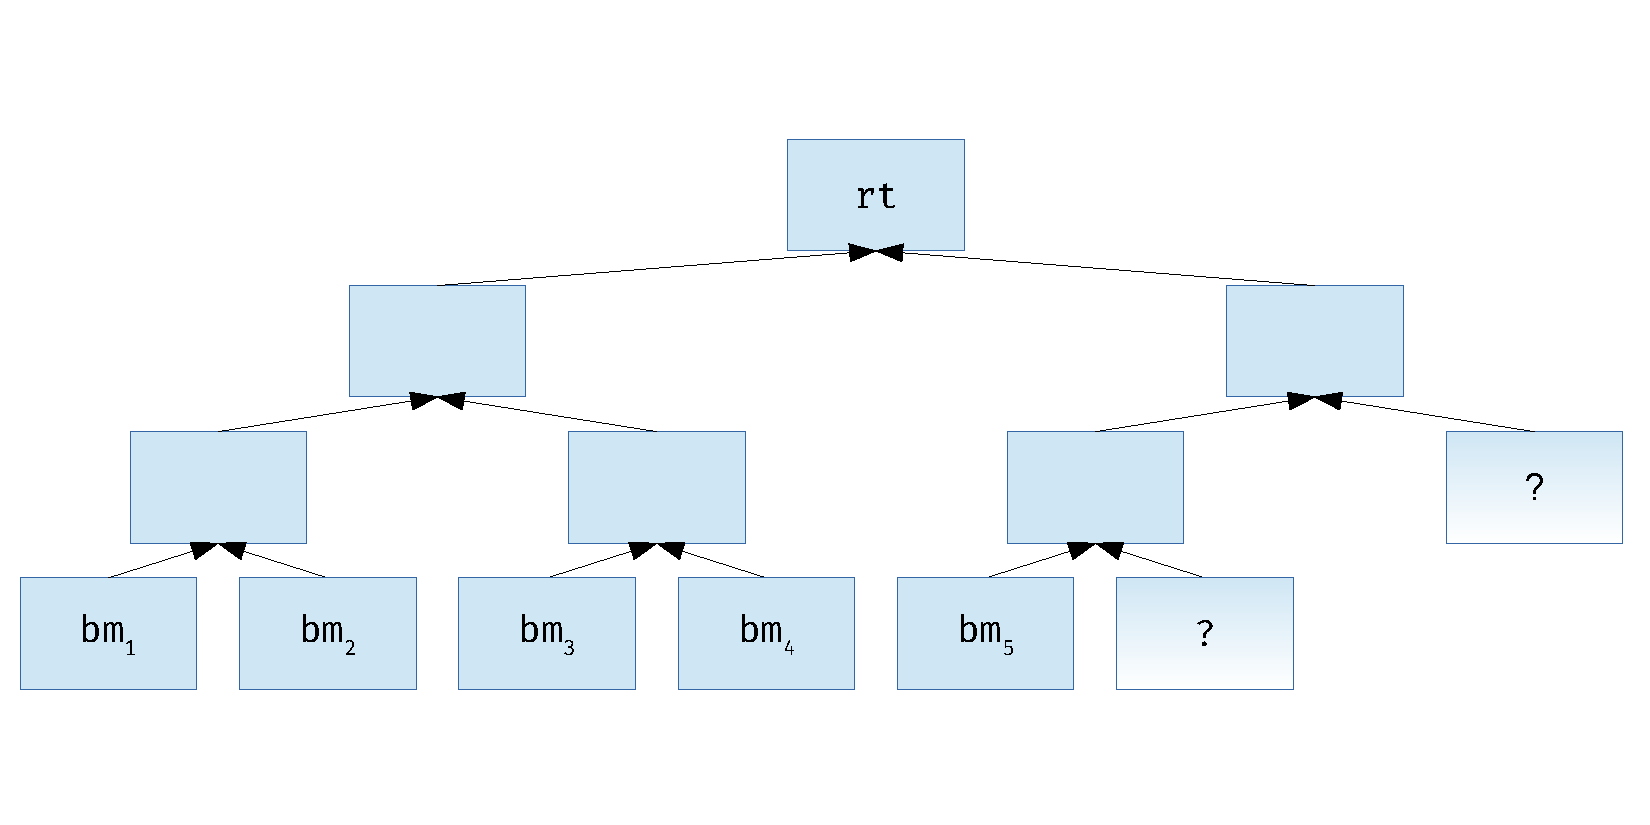
\includegraphics[scale=.4]{incremental_merkle}
\end{center}

The \coinCommitmentTree is an \incrementalMerkleTree of depth $\MerkleDepth$ used to
store \coinCommitments that \PourTransfers produce. Just as the \term{unspent
transaction output set} (UTXO) used in Bitcoin, it is used to express the existence
of value and the capability to spend it. However, unlike the UTXO, it is \emph{not}
the job of this tree to protect against double-spending, as it is append-only.

Blocks in the blockchain are associated (by all nodes) with the root of this tree
after all of its constituent \PourDescriptions' \coinCommitments have been
entered into the tree associated with the previous block.

\subsection{Spent Serials Map}

Transactions insert \serialNumbers into a \spentSerialsMap which is maintained 
alongside the UTXO by all nodes.

\eli{a tx is just a string, so it doesn't insert anything. Rather, nodes process 
tx's and the ``good'' ones lead to the addition of serials to the spent serials 
map.}

Transactions that attempt to insert a \serialNumber into this map that already
exists within it are invalid as they are attempting to double-spend.

\eli{After defining \term{transaction}, one should define what a \term{legal tx} is
(this definition depends on a particular blockchain [view]) and only then can one
talk about ``attempts'' of transactions, and insertions of serial numbers into the
spent serials map.}

\subsection{The Blockchain}

At a given point in time, the \blockchainview of each \fullnode consists of a
sequence of one or more valid \blocks. Each \block consists of a sequence of one or
more \transactions. In a given node's \blockchainview, \treestates are chained in an
obvious way:

\begin{itemize}
  \item The input \treestate of the first \block is the empty \treestate.
  \item The input \treestate of the first \transaction of a \block is the final
        \treestate of the immediately preceding \block.
  \item The input \treestate of each subsequent \transaction in a \block is the
        output \treestate of the immediately preceding \transaction.
  \item The final \treestate of a \block is the output \treestate of its last
        \transaction.
\end{itemize}

An \anchor is a Merkle tree root of a \treestate, and uniquely identifies that
\treestate given the assumed security properties of the Merkle tree's hash function.

Each \transaction is associated with a \sequenceOfPourDescriptions.
\todo{They also have a transparent value flow that interacts with the Pour
\changed{$\vpubOld$ and} $\vpubNew$.}
Inputs and outputs are associated with a value.

The total value of the outputs must not exceed the total value of the inputs.

The \anchor of the \changed{first} \PourDescription in a \transaction must refer to
some earlier \block's final \treestate.

\changed{
The \anchor of each subsequent \PourDescription may refer either to some earlier
\block's final \treestate, or to the output \treestate of the immediately preceding
\PourDescription.
}

These conditions act as constraints on the blocks that a \fullnode will
accept into its \blockchainview.

We rely on Bitcoin-style consensus for \fullnodes to eventually converge on their 
views of valid \blocks, and therefore of the sequence of \treestates in those 
\blocks.


\subparagraph{Value pool}

Transaction inputs insert value into a \term{value pool}, and transaction outputs 
remove value from this pool. The remaining value in the pool is available to miners 
as a fee.

\section{Pour Transfers and Descriptions}

A \PourDescription is data included in a \block that describes a \PourTransfer,
i.e. a confidential value transfer. This kind of value transfer is the primary
\Zerocash-specific operation performed by transactions; it uses, but should not be
confused with, the \PourCircuit used for the \zkSNARK proof and verification.

A \PourTransfer spends $\NOld$ \coins $\cOld{1..\NOld}$ and creates $\NNew$ \coins
$\cNew{1..\NNew}$. \Zcash transactions have an additional field $\vpour$, which is
a \sequenceOfPourDescriptions.

Each \PourDescription consists of:

\begin{list}{}{}
\changed{
\item $\vpubOldField$ which is a value $\vpubOld$ that the \PourTransfer removes
from the value pool.
}

\item $\vpubNewField$ which is a value $\vpubNew$ that the \PourTransfer inserts
into the value pool.

\item $\anchorField$ which is a merkle root $\rt$ of the \coinCommitmentTree at
some block height in the past, or the merkle root produced by a previous pour in
this transaction. \sean{We need to be more specific here.}

\item $\scriptSig$ which is a \script that creates conditions for acceptance of a
\PourDescription in a transaction.

\item $\scriptPubKey$ which is a \script used to satisfy the conditions of the
$\scriptSig$.

\item $\serials$ which is an $\NOld$ size sequence of serials $\snOld{\mathrm{1}..\NOld}$.

\item $\commitments$ which is a $\NNew$ size sequence of \coinCommitments 
$\cmNew{\mathrm{1}..\NNew}$.

\changed{
\item $\ephemeralKey$ which is a Curve25519 public key $\EphemeralPublic$.
}

\item $\ciphertexts$ which is a $\NNew$ size sequence of ciphertext components.
(\changed{$\ephemeralKey$ and} $\ciphertexts$ together form the \coinsCiphertext.)

\item $\vmacs$ which is a $\NOld$ size sequence of message authentication tags
$\h{\mathrm{1}..\NOld}$ that bind $\hSig$ to each $\SpendAuthorityPrivate$ of the
$\PourDescription$.

\item $\zkproof$ which is the zero-knowledge proof $\PourProof$.

\end{list}

\subparagraph{Computation of $\hSig$}

\newsavebox{\hsigbox}
\begin{lrbox}{\hsigbox}
\begin{bytefield}[bitwidth=0.045em]{808}
	\bitbox{80}{$\hSigInputVersionByte$} &
	\bitbox{256}{256 bit $\snOld{0}$} &
	\bitbox{24}{...} &
	\bitbox{256}{256 bit $\snOld{\NOld-1}$} &
	\bitbox{256}{$\scriptPubKey$}
\end{bytefield}
\end{lrbox}

Given a \PourDescription, we define:

\begin{itemize}
  \item[] $\hSig := \FullHashbox{\hsigbox}$
\end{itemize}

\subparagraph{Merkle root validity}

A \PourDescription is valid if $\rt$ is a \coinCommitmentTree root found in 
either the blockchain or a merkle root produced by inserting the \coinCommitments 
of a previous $\PourDescription$ in the transaction to the \coinCommitmentTree 
identified by that previous $\PourDescription$'s $\anchor$.

\subparagraph{Non-malleability}

A \PourDescription is valid if the script formed by appending $\scriptPubKey$ to 
$\scriptSig$ returns $true$. The $\scriptSig$ is cryptographically bound to 
$\PourProof$.

\subparagraph{Balance}

A \PourTransfer can be seen, from the perspective of the transaction, as
an input \changed{and an output simultaneously}.
\changed{$\vpubOld$ takes value from the value pool and}
$\vpubNew$ adds value to the value pool. As a result, \changed{$\vpubOld$ is
treated like an \emph{output} value, whereas} $\vpubNew$ is treated like an
\emph{input} value.

\changed{
Note that unlike original \Zerocash \cite{ZerocashOakland}, \Zcash does not have
a distinction between Mint and Pour transfers. The addition of $\vpubOld$ to a
\PourDescription subsumes the functionality of Mint. Also, \PourDescriptions
are indistinguishable regardless of the number of real input \coins.
}

\subparagraph{Commitments and Serials}

A \transaction that contains one or more \PourDescriptions, when entered into the 
blockchain, appends to the \coinCommitmentTree with all constituent 
\coinCommitments. All of the constituent \serialNumbers are also entered into the 
\spentSerialsMap of the \blockchainview \emph{and} \mempool. A \transaction is not 
valid if it attempts to add a \serialNumber to the \spentSerialsMap that already 
exists in the map.

\subsection{Pour Circuit and Proofs}

In \Zcash, $\NOld$ and $\NNew$ are both $2$.

A valid instance of $\PourProof$ assures that given a \term{primary input}
$(\rt, \snOld{\mathrm{1}..\NOld}, \cmNew{\mathrm{1}..\NNew}, \changed{\vpubOld,\;}
\vpubNew, \hSig, \h{1..\NOld})$, a witness of \term{auxiliary input}
$(\treepath{1..\NOld}, \cOld{1..\NOld}, \SpendAuthorityPrivateOld{\mathrm{1}..\NOld},
\cNew{1..\NNew}, \CoinAddressPreRand)$ exists, where:

\begin{list}{}{}

\item for each $i \in \{1..\NOld\}$: $\cOld{i}$ = $(\SpendAuthorityPublicOld{i},
\vOld{i}, \CoinAddressRandOld{i}, \CoinCommitRandOld{i})$

\item for each $i \in \{1..\NNew\}$: $\cNew{i}$ = $(\SpendAuthorityPublicNew{i},
\vNew{i}, \CoinAddressRandNew{i}, \CoinCommitRandNew{i})$

\item The following conditions hold:

\end{list}

\subparagraph{Merkle path validity}

for each $i \in \{1..\NOld\}$ \changed{$\mid$ $\vOld{i} \neq 0$}: $\treepath{i}$ must be a valid path
of depth $\MerkleDepth$ from \linebreak $\CoinCommitment{\cOld{i}}$ to Coin 
commitment merkle tree root $\rt$.

\subparagraph{Balance}

$\changed{\vpubOld +} \vsum{i=1}{\NOld} \vOld{i} = \vpubNew + \vsum{i=1}{\NNew} \vNew{i}$.

\subparagraph{Serial integrity}

for each $i \in \{1..\NNew\}$: 
$\snOld{i} = \PRFsn{\SpendAuthorityPrivateOld{i}}(\CoinAddressRandOld{i})$.

\subparagraph{Spend authority}

for each $i \in \{1..\NOld\}$:
$\SpendAuthorityPublicOld{i} = \PRFaddr{\SpendAuthorityPrivateOld{i}}(0)$.

\subparagraph{Non-malleability}

for each $i \in \{1..\NOld\}$: $\h{i}$ = $\PRFpk{\SpendAuthorityPrivateOld{i}}(i, \hSig)$

\subparagraph{Uniqueness of $\CoinAddressRandNew{i}$}

for each $i \in \{1..\NNew\}$: $\CoinAddressRandNew{i}$ = $\PRFrho{\CoinAddressPreRand}(i, \hSig)$

\subparagraph{Commitment integrity}

for each $i \in \{1..\NNew\}$: $\cmNew{i}$ = $\CoinCommitment{\cNew{i}}$

\section{Encoding Addresses, Private keys, Coins, and Pour descriptions}

This section describes how \Zcash encodes public addresses, private keys,
coins, and \PourDescriptions.

Addresses, keys, and coins, can be encoded as a byte string; this is called
the \term{raw encoding}. This byte string can then be further encoded using
Base58Check. The Base58Check layer is the same as for upstream \Bitcoin
addresses \cite{Base58Check}.

SHA-256 compression function outputs are always represented as strings of 32
bytes.

The language consisting of the following encoding possibilities is prefix-free.

\subsection{Transparent Public Addresses}

These are encoded in the same way as in \Bitcoin \cite{Base58Check}.

\subsection{Transparent Private Keys}

These are encoded in the same way as in \Bitcoin \cite{Base58Check}.

\subsection{Confidential Public Addresses}

A \publicAddress consists of $\SpendAuthorityPublic$ and $\TransmitPublic$.
$\SpendAuthorityPublic$ is a SHA-256 compression function output.
$\TransmitPublic$ is a \changed{Curve25519} public key, for use with the
encryption scheme defined in section ``In-band secret distribution".

\subsubsection{Raw Encoding}

The raw encoding of a confidential address consists of:

\begin{equation*}
\begin{bytefield}[bitwidth=0.07em]{520}
    \bitbox{48}{\changed{$\PublicAddressLeadByte$}} &
    \bitbox{256}{$\SpendAuthorityPublic$ (32 bytes)} &
    \bitbox{256}{A \changed{32-byte} encoding of $\TransmitPublic$}
\end{bytefield}
\end{equation*}

\begin{itemize}
\changed{
    \item A byte, $\PublicAddressLeadByte$, indicating this version of the
        raw encoding of a \Zcash public address.
}
    \item 32 bytes specifying $\SpendAuthorityPublic$.
    \item \changed{32 bytes} specifying $\TransmitPublic$, \changed{using the
        normal encoding of a Curve25519 public key \cite{Curve25519}}.
\end{itemize}

\daira{check that this lead byte is distinct from other Bitcoin stuff,
and produces `z' as the Base58Check leading character.}

\nathan{what about the network version byte?}

\subsection{Confidential Address Secrets}

A confidential address secret consists of $\SpendAuthorityPrivate$ and
$\TransmitPrivate$. $\SpendAuthorityPrivate$ is a SHA-256 compression function
output. $\TransmitPrivate$ is a \changed{Curve25519} private key, for use with
the encryption scheme defined in section ``In-band secret distribution".

\subsubsection{Raw Encoding}

The raw encoding of a confidential address secret consists of, in order:

\begin{equation*}
\begin{bytefield}[bitwidth=0.07em]{520}
    \bitbox{48}{\changed{$\PrivateAddressLeadByte$}} &
    \bitbox{256}{$\SpendAuthorityPrivate$ (32 bytes)} &
    \bitbox{256}{$\TransmitPrivate$ (32 bytes)}
\end{bytefield}
\end{equation*}

\begin{itemize}
\changed{
    \item A byte $\PrivateAddressLeadByte$ indicating this version of the
        raw encoding of a \Zcash private key.
}
    \item 32 bytes specifying $\SpendAuthorityPrivate$.
    \item 32 bytes specifying $\TransmitPrivate$.
\end{itemize}

\daira{check that this lead byte is distinct from other Bitcoin stuff,
and produces `z' as the Base58Check leading character.}

\nathan{what about the network version byte?}

\subsection{Coins}

Transmitted coins are stored on the blockchain in encrypted form, together with
a \coinCommitment $\cm$.

The \coinPlaintexts associated with a \PourDescription are encrypted to the
respective \transmitPublicAlgorithm keys $\TransmitPublicNew{\mathrm{1}..\NNew}$,
and the result forms a \coinsCiphertext.

Each \coinPlaintext consists of $(\Value, \CoinAddressRand, \CoinCommitRand\changed{, \Memo})$,
where:

\begin{itemize}
    \item $\Value$ is a 64-bit unsigned integer representing the value of the
        \coin in \zatoshi (1 \ZEC = $10^8$ \zatoshi).
    \item $\CoinAddressRand$ is a 32-byte $\PRFsn{\SpendAuthorityPrivate}$ preimage.
    \item $\CoinCommitRand$ is a 48-byte \COMMtrapdoor.
\changed{
    \item $\Memo$ is a 64-byte \memo associated with this \coin.
}
\end{itemize}

\changed{
The usage of the $\memo$ is by agreement between the sender and recipient of the
\coin. It should be encoded as a UTF-8 human-readable string \cite{Unicode}, padded
with zero bytes. Wallet software is expected to strip any trailing zero bytes and
then display the resulting UTF-8 string to the recipient user, where applicable.
Incorrect UTF-8-encoded byte sequences should be displayed as replacement characters
(\ReplacementCharacter). This does not preclude uses of the \memo by automated
software, but specification of such usage is not in the scope of this document.
}

Note that the value $\CoinCommitS$ described as being part of a \coin in the
\Zerocash paper is not encoded because the instantiation of $\COMM{\CoinCommitS}$
does not use it.

\subsection{Raw Encoding}

The raw encoding of a \coinPlaintext consists of, in order:

\begin{equation*}
\begin{bytefield}[bitwidth=0.035em]{1224}
    \bitbox{80}{\changed{$\TransmitPlaintextVersionByte$}} &
    \bitbox{144}{$\Value$ (8 bytes)} &
    \bitbox{256}{$\CoinAddressRand$ (32 bytes)} &
    \bitbox{384}{$\CoinCommitRand$ (48 bytes)} &
    \changed{\bitbox{512}{$\Memo$ (64 bytes)}}
\end{bytefield}
\end{equation*}

\begin{itemize}
\changed{
    \item A byte $\TransmitPlaintextVersionByte$ indicating this version of the raw 
encoding of a \coinPlaintext.
}
    \item 8 bytes specifying a big-endian encoding of $\Value$.
    \item 32 bytes specifying $\CoinAddressRand$.
    \item 48 bytes specifying $\CoinCommitRand$.
\changed{
    \item 64 bytes specifying $\Memo$.
}
\end{itemize}

\section{Pours (within a transaction on the blockchain)}

TBD.

\changed{Describe case where there are fewer than $\NOld$ real input coins.}

\section{Transactions}

TBD.


\changed{
\section{Differences from the Zerocash paper}

\begin{itemize}
    \item Instead of ECIES, we use an encryption scheme based on $\CryptoBox$,
defined in section ``In-band secret distribution".
    \item Faerie Gold fix (TBD).
    \item The paper defines a coin as a tuple $(\SpendAuthorityPublic, \Value,
\CoinAddressRand, \CoinCommitRand, \CoinCommitS, \cm)$, whereas this specification
defines it as $(\SpendAuthorityPublic, \Value, \CoinAddressRand, \CoinCommitRand)$.
This is just a clarification, because the instantiation of $\COMM{\CoinCommitS}$
in section 5.1 of the paper does not use $\CoinCommitS$, and $\cm$ can be computed
from the other fields.
\end{itemize}
}


\section{References}

\begingroup
\renewcommand{\section}[2]{}
\bibliographystyle{plain}
\bibliography{zcash}
\endgroup

\end{document}
